\section{Realisierung}
\label{sec:Realisierung}

Wie im Anhang (\secref{sec:Entscheidung-Programmiersprache}) beschrieben und begründet, wird \texttt{px} mit \textsc{Go} umgesetzt. Da die Standard Library von \textsc{Go} sehr umfassend ist, die mit dem Package \texttt{net/http} über einen mächtigen HTTP-Client (und Server) verfügt, wird nur eine Fremdkomponente (Zugriff auf den Keystore) eingesetzt.

Enorm hilfreich in der Umsetzung war Standardwerk zu \textsc{Go} \cite{gopl}, das nicht nur die Programmiersprache beschreibt, sondern auch deren idiomatischen Gebrauch.

\subsection{Architektur: Package-Übersicht}

\textsc{Go}-Code wird in sogenannte Packages aufgeteilt. Da das Projekt in \textsc{GitLab} \texttt{px} heisst, wird das Hauptpackage als \texttt{px} benannt. Im Root-Verzeichnis befindet sich kein \textsc{Go}-Code.\footnote{\texttt{px.go} beinhaltet bloss eine Package-Deklaration mit einem entsprechenden Kommentar.} Dieser ist in verschiedenen Unterverzeichnissen (\texttt{requests}, \texttt{tokenstore}, usw.) abgelegt. Die Dateien in den Unterpackages deklarieren ihre Packagezugehörigkeit jeweils mit dem unmittelbaren Überverzeichnis, also beispielsweise nicht \texttt{px/tokenstore}, sondern nur \texttt{tokenstore}. Bei der Verwendung der Packages hingegen wird der ganze Pfad angegeben: \texttt{px/tokenstore}.

Der Code für das ausführbare Programm (\texttt{px.go}) befindet sich gemäss Konvention\footnote{\url{https://github.com/golang-standards/project-layout\#cmd}} im \texttt{cmd}-Unterverzeichnis \cite[S. 12]{powerful-cli-apps-in-go}. Das Package heisst jedoch nicht \texttt{cmd}, sondern \texttt{main}, und verfügt über eine Funktion namens \texttt{main} als Haupteinstiegspunkt. Somit ist \texttt{px} als Library, und \texttt{cmd/px.go} als Client dieser Library zu verstehen.\footnote{Da sich nur knapp ein Viertel des Programmcodes im Client-Teil befinden, könnte auf Basis der \texttt{px}-Library recht einfach ein alternativer Client umgesetzt werden.} Die Projektstruktur ist auf der linken Seite der \imgref{img:Komponentendiagramm} zu sehen. Die einzelnen Packages haben folgende Verantwortlichkeiten:

\begin{figure}
    \centering
    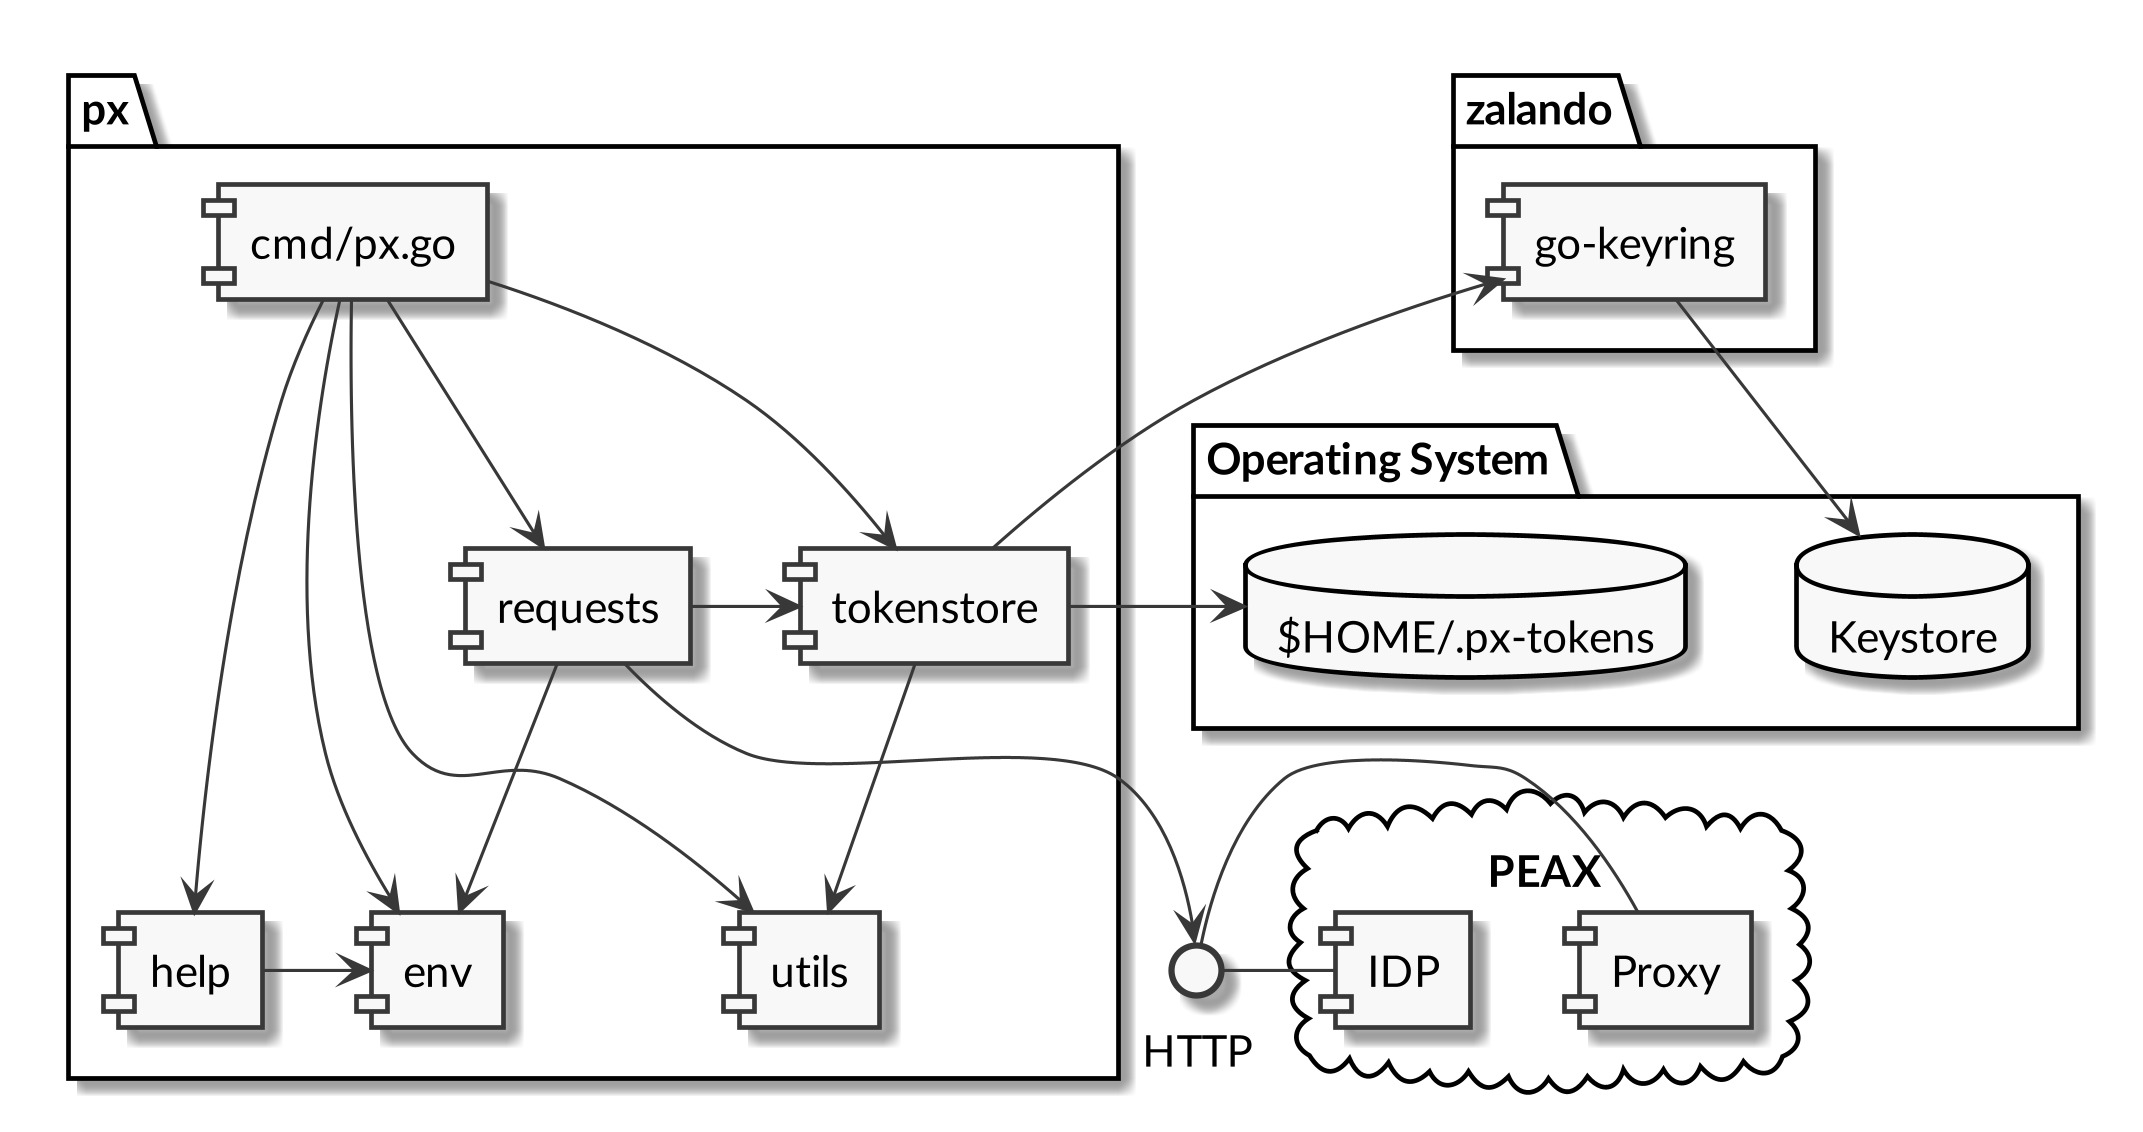
\includegraphics[width=\linewidth]{pics/komponentendiagramm.png}
    \caption{Die Package-Struktur von \texttt{px} (Komponentendiagramm)}
    \label{img:Komponentendiagramm}
\end{figure}

\begin{description}
    \item[\texttt{env}] Die Umgebungen (\secref{sec:Umgebungen}) sind in diesem Package aufgelistet. Jede Umgebung verfügt über ein URL-Schema, womit (via Proxy) auf das Backend und direkt auf den IDP zugegriffen werden kann. Verschiedene Funktionen bieten die Möglichkeit, URLs für den Ressourcenzugriff anhand der jeweiligen Umgebung und weiterer Parameter zu erzeugen, was mit dem Unit Test \texttt{env\_test.go} überprüft wird. Die Standardeinstellung, welcher Keystore (sicher/unsicher) zu verwenden ist, wird statisch pro Umgebung definiert.
    \item[\texttt{help}] Dieses Package umfasst die Hilfetexte. Zu jedem Befehl gibt es jeweils eine kurze, einzeilige Beschreibung, und einen ausführlichen Hilfetext. Dieses Package importiert das \texttt{env}-Package, damit bei der Hilfe zum Login-Befehl (\texttt{px login}) die verfügbaren Umgebungen automatisch aufgelistet werden können.
    \item[\texttt{tokenstore}] Hier sind zentrale Datenstrukturen für das Token-Handling mit dazugehörigen Funktionen definiert. Die Datenstruktur \texttt{TokenPair} dient zur lokalen, persistenten Speicherung von Tokens. Sie wird auf Basis einer \texttt{TokenResponse} aufgebaut, indem Informationen extrahiert und anhand von Kontextinformationen ergänzt. Die Datenstruktur \texttt{TokenStore} speichert pro Umgebung und Token-Typ (\texttt{agent}, \texttt{user}) ein \texttt{TokenPair} ab. Der \texttt{TokenStore} wird als JSON-Struktur serialisiert und im \texttt{\$HOME}-Verzeichnis des Benutzers abgespeichert. Der Zugriff auf den sicheren Keystore ist ebenfalls hier implementiert.
    \item[\texttt{requests}] In diesem Package sind die eigentlichen Zugriffe auf die API via HTTP umgesetzt. Hier sind Datenstrukturen für die Credential-Payloads mit dazugehörigen Funktionen definiert, die für Login-Vorgänge verwendet werden (\texttt{credentials.go}. Für die verschiedenen Befehle (\texttt{login}, \texttt{get}, \texttt{upload} usw.) sind hier dazugehörige Funktionen definiert. Der transparente Retry-Mechanismus ist ebenfalls hier implementiert (\texttt{requests.go}). Das Package \texttt{tokenstore} wird verwendet, um die Requests mit den notwendigen Authentifizierungsinformationen (\texttt{Authentication}-Header) auszustatten.
    \item[\texttt{utils}] Dieses Package umfasst verschiedene Funktionen, die von verschiedenen anderen Packages und vom Hauptprogramm verwendet werden, jedoch nicht direkt zu den jeweiligen anderen Packages gehören. Die Eingabeaufforderung für Passwörter (sicher über ein SSH-Terminal, d.h. ohne Echo) ist etwa hier umgesetzt (\texttt{pwinput.go} und \texttt{pwinput\_windows.go}\footnote{Aufgrund eines offenen Fehlers (\url{https://github.com/golang/go/issues/34461}) funktioniert die sichere Passworteingabe nicht unter \textsc{Windows}. Aus diesem Grund wird mithilfe eines Build Constraints (\url{https://golang.org/pkg/go/build/\#hdr-Build\_Constraints}) für den \textsc{Windows}-Build eine unsichere Variante, für alle anderen Betriebssysteme die sichere Variante verwendet.}). Weiter gibt es Funktionen zum automatischen Ermitteln des MIME-Types einer Datei, und eine Funktion zur rekursiven Auflisten lesbarer Dateien in einem Unterverzeichnis.
    \item[\texttt{cmd/px.go}] Dies ist der eigentliche Command Line Client mit der Einstiegsfunktion \texttt{main}. Die zur Verfügung stehenden Befehle weden in einer Map namens \texttt{commands} abgespeichert, wobei der Befehlsname den Key bildet, und der Wert eine Datenstruktur bestehend aus einer Funktionsreferenz, dem einzeiligen Infotext und dem längeren Hilfetext (siehe Package \texttt{help}) zusammengesetzt ist. Die \texttt{main}-funktion prüft, ob der eingegebene Befehl in der Map gefunden wurde, und führt diese dann aus. Jede dieser Command-Funktionen nimmt den \texttt{TokenStore} als Argument entgegen, und gibt einen optionalen Fehler zurück.\footnote{Die Befehle \texttt{help} und \texttt{env} bilden eine Ausnahme.} Der \texttt{TokenStore} wird zu Beginn von \texttt{main} aus \texttt{~/.px-tokens} geladen, und am Ende (mit möglichen Änderungen) wieder in diese Datei zurückgeschrieben.\footnote{Die sicher verwahrten Tokens werden bei Bedarf, d.h. bei einem entsprechenden Request, nachgeladen.} Die einzelnen Command-Funktionen sind selber für ihre Seiteneffekte (Ausgabe möglicher Payloads) verantwortlich. Die Fehlerausgabe wird über die Rückgabe eines Fehlers in \texttt{main} abgehandelt. Die Flags sind ebenfalls für jeden Befehl eigens definiert, wobei Gemeinsamkeiten in Hilfsfunktionen und Konstanten (Beschreibungstexte) ausgelagert sind. Das Parsen der Kommandozeilenargumente wird vom sehr mächtigen und komfortablen \texttt{flag}-Package übernommen, das Teil der Standard Library von \textsc{Go} ist. Tritt bei der Programmausführung ein Fehler auf, wird einerseits eine Fehlermeldung auf \texttt{stderr} geschrieben, andererseits der Rückgabewert \texttt{1} an den aufrufenden Prozess zurückgegeben.\footnote{Im Gegensatz zu \texttt{0}, das für eine erfolgreiche Ausführung steht.} Dieser Rückgabecode wird in den Testskripts über die Shell-Variable \texttt{\$?} geprüft.
\end{description}

\subsection{Zwei-Faktor-Authentifizierung}

Hat ein Benutzer im Portal die Zwei-Faktor-Authentifizierung über SMS oder TOTP aktiviert, wird der initiale Login-Request mit Benutzername und Passwort mit dem HTTP-Status 380 quittiert. Diese Antwort enthält auch die Information, welcher zweite Faktor (SMS oder TOTP) verlangt wird.

Dem Benutzer wird eine entsprechende Eingebeaufforderung angezeigt. Nach der Eingabe wird der initiale Request mit dem eingegebenen zweiten Faktor ergänzt und erneut an den IDP gesendet. Hat der Vorgang funktioniert, erhält der Benutzer das Token-Pair, das im Keystore für die spätere Verwendung abgelegt wird.

Dieser Vorgang ist in \imgref{fig:2fa} mit einem Sequenzdiagramm veranschaulicht.

\begin{figure}
    \centering
    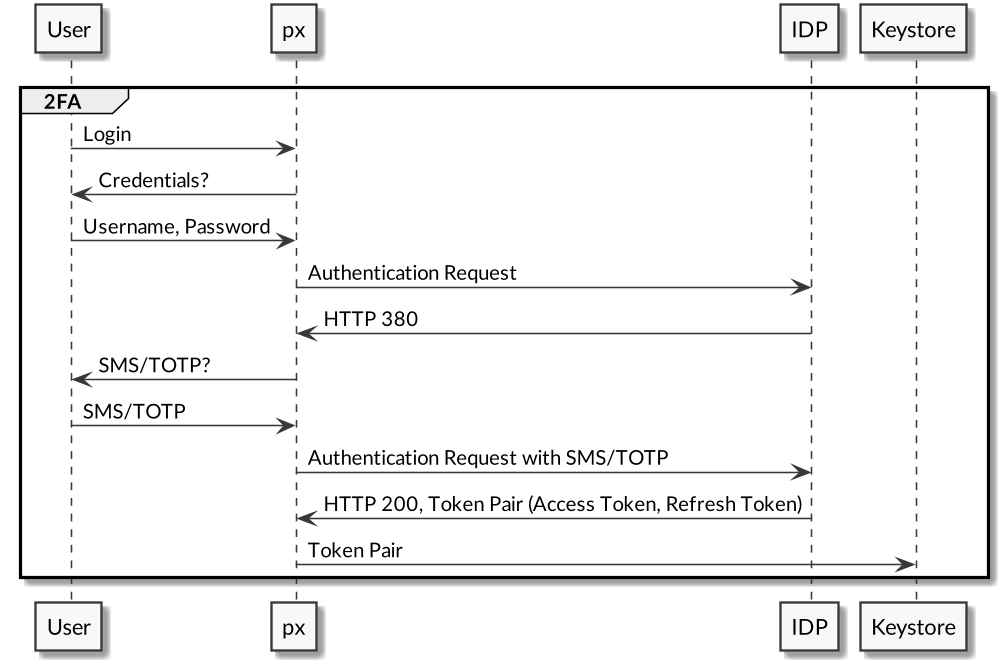
\includegraphics[width=\linewidth]{pics/sequence-2fa.png}
    \caption{Der Ablauf der Zwei-Faktor-Authentifizierung mit SMS oder OTP (Sequenzdiagramm)}
    \label{fig:2fa}
\end{figure}

\subsection{Token Store}
\label{sec:Realisierung-Token-Store}

Für jede Umgebung ist mit dem Flag \texttt{Confidential} definiert, ob die Tokens standardmässig sicher oder unsicher verwahrt werden sollen. Wie im Abschnitt \secref{sec:Konzept-Token-Store} beschrieben kann diese Einstellung mit den entsprechenden Flags übersteuert werden.

Wurde die unsichere Variante gewählt bzw. beibehalten, werden die beiden Tokens direkt in die JSON-Struktur geschrieben, die vor Beendigung des Clients nach \texttt{~/.px-tokens} geschrieben wird. Für jede Kombination von Token-Art (\texttt{user} oder \texttt{agent}) und Umgebung (\texttt{test}, \texttt{stage} usw.) wird je ein Feld \texttt{refresh\_token} und \texttt{access\_token} gespeichert. Als zusätzliches Feld wird \texttt{use\_keystore} mit dem Wert \texttt{false} abgespeichert.

Wird jedoch die sichere Variante gewählt bzw. beibehalten, wird unter der Kombination von Token-Art und Umgebung kein Token Pair abgespeichert, sondern bloss das Feld \texttt{use\_keystore} mit dem Wert \texttt{true}, was bei künftigen Token-Zugriffen als Verweis auf den nativen Keystore zu verstehen ist.

Das folgende Codebeispiel zeigt einen verkürzten Auszug aus der Datei \texttt{~/.px-tokens}, wobei für die Umgebung \texttt{test} die unsichere und für die Umgebung \texttt{stage} die sichere Token-Verwahrung verwendet worden ist.

\begin{lstlisting}[caption={Die JSON-Struktur für den Keystore (Auszug)}]
{
	"tokens": {
		"user_test": {
			"access_token": "eyJhbGciOiJSUz...",
			"refresh_token": "eyJhbGciOiJIUz...",
			"use_keystore": false
		},
		"user_stage": {
			"use_keystore": true
		}
	},
	"default_environment": "stage"
}
\end{lstlisting}

Der sichere Keystore ist als Key-Value-Store mit globalem Namensraum zu verstehen. Die Keys müssen also vollständig qualifiziert sein, d.h. alle Informationen enthalten, die etwa einen Refresh Token von \texttt{px} für einen Benutzer auf der Umgebung \texttt{prod} von einem auf dem Computer hinterlegten E-Mail-Passwort oder dergleichen unterscheidet. Hierzu wurde das folgende Namensschema (Zeile 1) gewählt:

\begin{lstlisting}[caption={Namensschema für die Keys auf dem nativen Keystore (mit Beispielen)},numbers=left]
px:[environment]:[(user|agent)]:[(refresh|access)Token]
px:test:user:refreshToken
px:prod:agent:accessToken
\end{lstlisting}

Zeile 2 zeigt den Key für einen Refresh Token für die User API auf der Umgebung \texttt{test}. Auf Zeile 3 ist ein Key für einen Access Token für die Agent API auf der Umgebng \texttt{prod} zu sehen.

\subsubsection{Fremdkomponente \texttt{zalando/go-keyring}}

Da sich der Zugriff auf den sicheren Keystore von Plattform zu Plattform unterscheidet, wurde dieser Mechanismus nicht selber implementiert. Das Package \texttt{go-keyring} von \textsc{Zalando}\footnote{\url{https://github.com/zalando/go-keyring}} löst dieses Problem bereits ‒ und funktionierte auf Anhieb.

Das Package \texttt{go-keyring} wird nur im Package \texttt{tokenstore} verwendet, und sonst nirgends in \texttt{px}. Mithilfe der Funktionen \texttt{keyring.Set}, \texttt{keyring.Get} und \texttt{keyring.Delete} kann Secret abgespeichert, gelesen und gelöscht werden. Zu jedem Key wird nicht nur ein Passwort (das eigentliche Secret), sondern auch ein Benutzername abgelegt. Als Passwort dient jeweils der Token. Als Benutzername wurde der Vollständigkeit halber der String \texttt{"px"} verwendet.\footnote{Für \texttt{px} spielt es keine Rolle, \textit{welcher} Benutzer eingeloggt ist. Validierungen auf den Scope zur Verhinderung von Fremdzugriffen werden serverseitig geprüft. Der Benutzer von \texttt{px} soll auch solche Zugriffe versuchen können, ohne schon clientseitig abgeblockt zu werden, um etwa Angriffe simulieren zu können.}

Diese drei Funktionen werden durch die eigenen Funktionen \texttt{storeSecret}, \texttt{loadSecret} und \texttt{deleteSecret} (\texttt{tokenstore/tokenpair.go}) gewrappt, wobei zusätzlich ein einheitliches Key-Format über die Funktion \texttt{tokenKeys} sichergestellt wird.

\subsection{Retry-Mechanismus}
\label{sec:Retry-Mechanismus}

Im Konzept (\secref{sec:Token-Refresh}) wurde beschrieben, nach welcher Strategie die Tokens aktualisiert werden sollen. Das Sequenzdiagramm \imgref{fig:retry-mechanism} zeigt, wie dies umgesetzt worden ist.

\begin{figure}
    \centering
    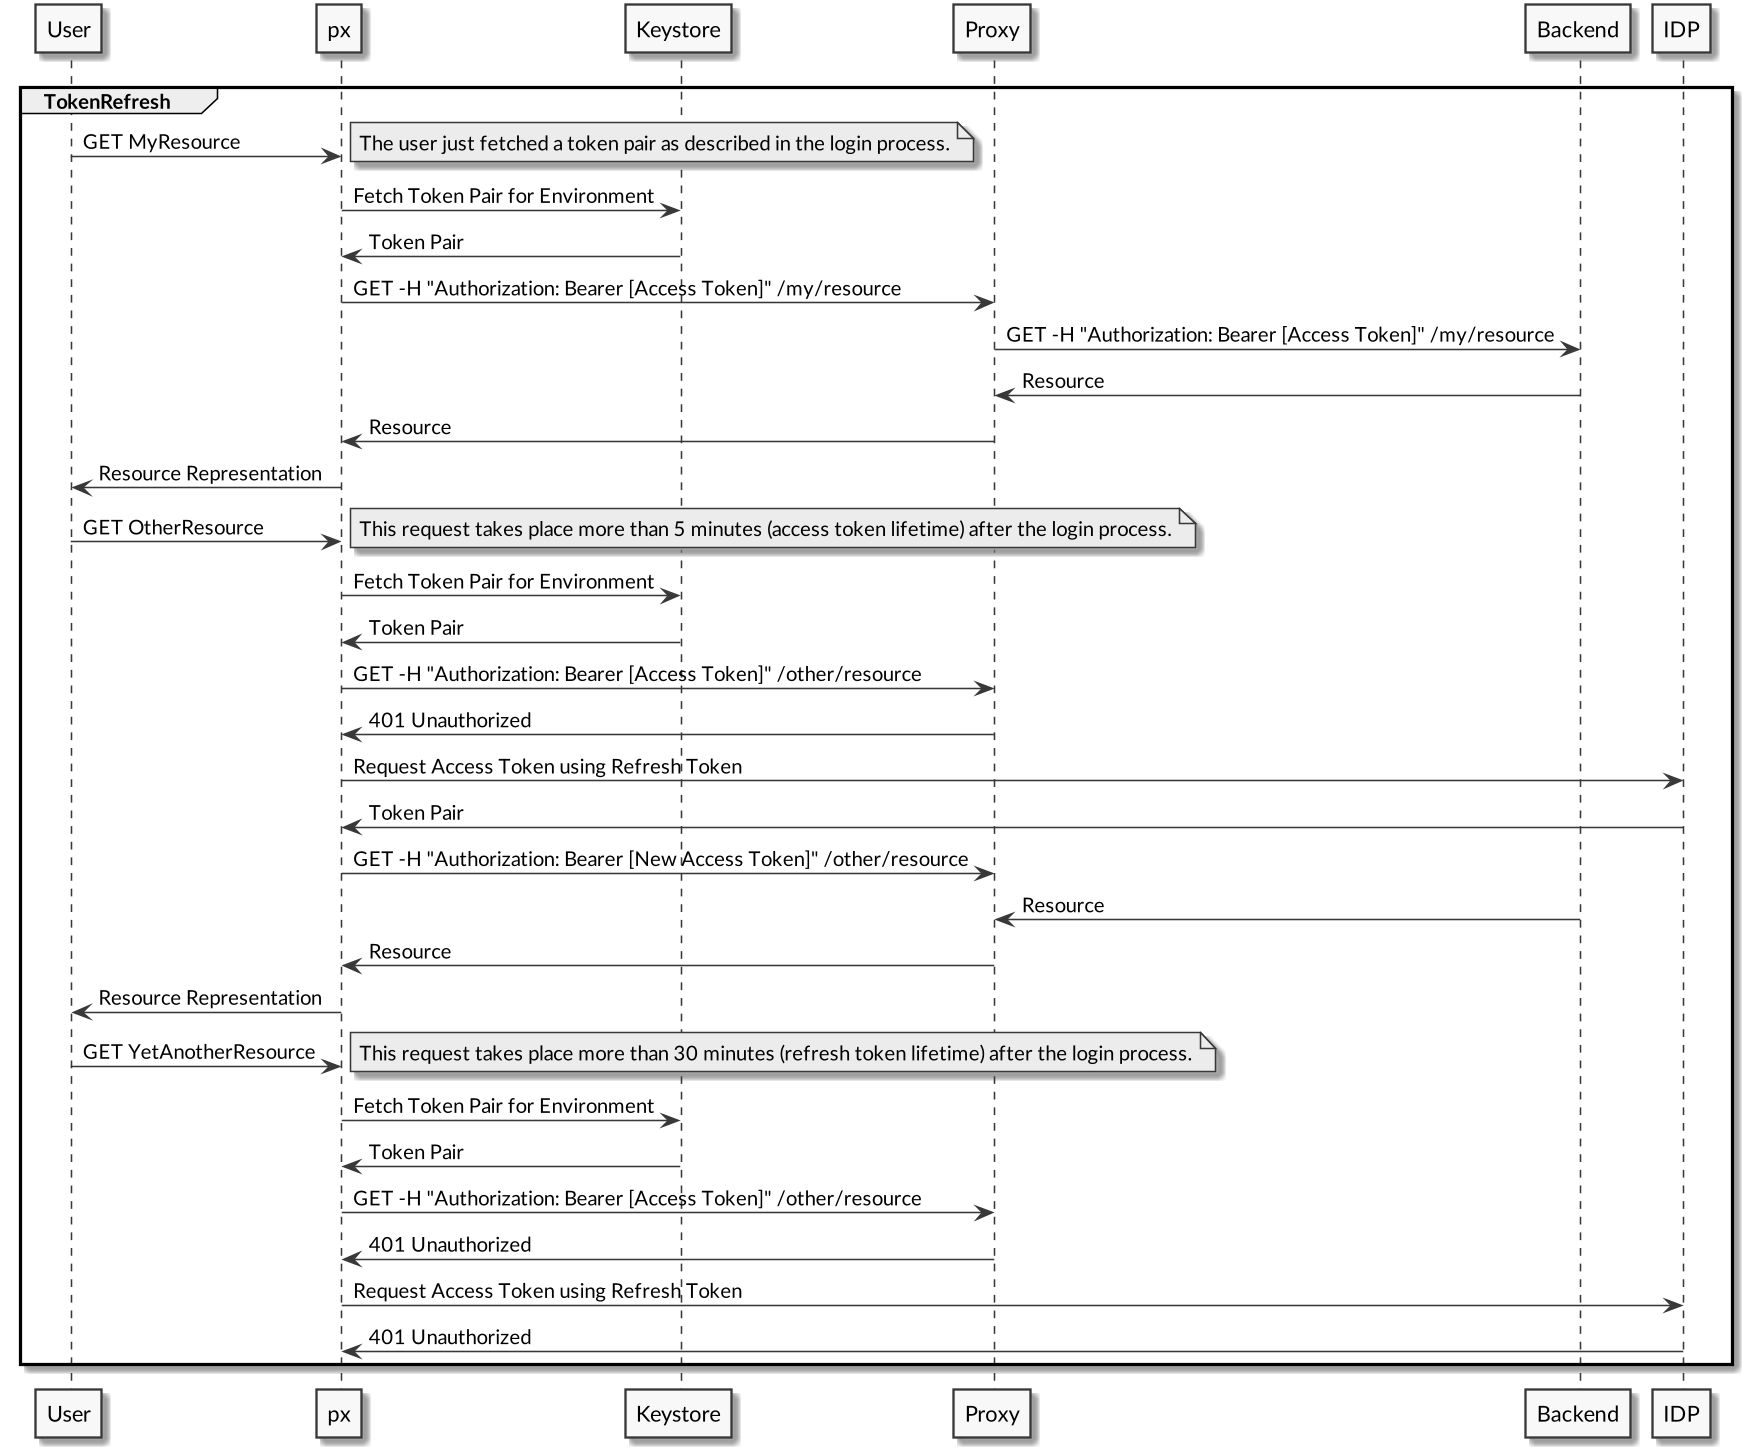
\includegraphics[width=\linewidth]{pics/sequence-retry.png}
    \caption{Der für den Benutzer transparente Retry-Mechanismus mit einem Token Pair, das im Hintergrund automatisch aktualisiert wird (Sequenzdiagramm)}
    \label{fig:retry-mechanism}
\end{figure}

Einige Implementierungsdetails, die auf dem Sequenzdiagramm nicht ersichtlich sind, sollen an dieser Stelle noch erläutert werden.

Der erste, naive Implementierungsversuch, der darin bestand, einen gescheiterten Request (mit HTTP-Status \texttt{401 Unauthorized}) mit aktualisiertem \texttt{Authorization}-Header einfach erneut abzuschicken, scheiterte für Requests, die über einen Body verfügen, was bei \texttt{POST}, \texttt{PUT} und \texttt{PATCH} der Fall ist. Grund dafür ist, dass die Repräsentation des Bodies bei einem ausgeführten Request konsumiert wird, und anschliessend nicht mehr verwendet werden darf.

Technisch war dies zunächst so implementiert worden, dass die Funktion \texttt{doWithToken\-Refresh} (\texttt{requests/requests.go}) als Parameter (nebst Kontextinformationen zum Auffinden der richtigen Tokens) einen Request erwartete. Die einzelnen Request-Funktionen (\texttt{Get}, \texttt{Post}, \texttt{Put}, \texttt{Patch} usw.) erstellten den initialen Request und übergaben ihn an \texttt{doWith\-Token\-Refresh}, welches dann anhand des Token Stores einen Token Refresh durchführte, und den initialen Request mit aktualisiertem \texttt{Authorization}-Header erneut abschickte.

Die Lösung für das Problem mit den konsumierten Bodies konnte gelöst werden, indem für jeden erneuten Versuch ein neuer Request aufgebaut wird. Da \texttt{doWithTokenRefresh} jedoch nicht über alle Informationen verfügen kann, welche zum Erstellen eines Requests nötig sind, musste ein Weg gefunden werden, diese Kontextinformationen für alle möglichen Arten von Requests mitliefern zu können. Da \textsc{Go} \textit{first class functions} unterstützt, konnte dies sehr elegant mit einer Closure gelöst werden \cite[S. 136]{gopl}. Die Client-Funktion übergibt nicht mehr einen Request, sondern eine Funktion, die einen Request erstellt. Die Kontextinformationen zur Erstellung des Requests erhält sie von der umschliessenden (\textit{enclosing}) Funktion; den aktualisierten Access Token erhält sie zu einem späteren Zeitpunkt als Parameter, nachdem \texttt{doWithTokenRefresh} das Token Pair aktualisiert hat.\footnote{Wäre \texttt{px} mit einer stark objektorientierten Programmiersprache wie \textsc{Java} oder \textsc{C++} umgesetzt worden, dürfte an dieser Stelle wohl ein Klassendiagramm mit \texttt{AbstractRequestFactory}, \texttt{GetRequestFactoryImpl} und dergleichen stehen. \textsc{Peter Norvig} hat demonstriert, dass in funktionalen Programiersprachen 16 der 23 \textsc{GoF}-Patterns \textit{«invisible or simpler»} sind (\url{http://www.norvig.com/design-patterns/design-patterns.pdf}). Die Implementierung von \texttt{doWithTokenRefresh} veranschaulicht dieses Prinzip.}

\subsection{Umgang mit Risiken}

Von den ermittelten Risiken (\secref{sec:Risikoanalyse} sind bei der Umsetzung v.a. die technischen und sicherheitsrelevanten Risiken relevant. Mit ihnen wurde folgendermassen verfahren:

\begin{description}
    \item[Token-Verwahrung] Mit dem nativen Keystore wurde eine Lösung gefunden, die so sicher ist, wie der Keystore des zugrundeliegenden Betriebssystems. Möchte der Benutzer von \texttt{px} die Tokens der Produktivumgebung im Klartext abspeichern, muss er das explizit angeben. Die Kombination aus sicheren Grundeinstellungen und der Möglichkeit, diese bei Bedarf zu übersteuern, hat der Anwender eine standardmässig sichere, jedoch ausreichend flexible Lösung.
    \item[Payment-Schnittstelle] Hat der Benutzer ein Bankkonto hinterlegt, und loggt er sich mit \texttt{px} auf das Produktivsystem ein, kann er Zahlungen mit den entsprechenden Requests in Auftrag geben. Es bestehen die gleichen Risiken wie bei der Bedienung des Portals. Auf eine unnötige und willkürliche Einschränkung der API-Abdeckung wurde verzichtet. Das Risiko liegt ganz beim Benutzer; die Sicherheit steht und fällt mit der Token-Verwahrung, welche sicher genug umgesetzt worden ist.
\end{description}

\subsection{Notizen zur Implementierung und zum Testing}

Während der Umsetzung von \texttt{px} wurden zu jeder User Story Umsetzungsnotizen und Testprotokolle geschrieben, die im Zusatzdokument \textit{Backlog} (\secref{apx:WeitereDokumente}) zu finden sind. Da dieses Dokument recht umfassend ist, ist es als Referenz zu lesen. Hierbei ist jedoch zu beachten, dass das Dokument, gerade die Auflistung der User Stories, historisch gewachsen ist: Notizen früherer Stories wurden teils durch Notizen späterer Stories obsolet gemacht. Es empfiehlt sich also, bei der Lektüre so weit unten wie möglich ‒ d.h. bei der jeweiligen Story, die von Interesse ist ‒ einzusteigen, und bei Unklarheiten weiter oben nachzulesen, um den Hintergrund besser erfassen zu können.

Aufgrund der agilen Vorgehensweise gibt es keine umfassenden Testpläne und Testprotokolle, zumal das Testen nicht als von der Implementierung getrennte Phase praktiziert worden ist. Eine Ausnahme bilden die wenigen manuellen Tests (Regressionstests), die ab Sprint 3 jeweils durchgeführt worden und am Ende des \textit{Backlog}-Dokuments verzeichnet sind.
